% !TEX root = top.tex
% above command is so that compilation is always from top.tex

\section{Background} \label{sec:design}

In this section we describe the platforms HyperFork is built upon, including an
overview of the KVM hypervisor and kvmtool virtual machine monitor.

\subsection{KVM Overview}

% TODO KVM is ......

A full KVM system contains a number of major components within a Linux host
machine, as depicted in Figure~\ref{fig:kvm-arch}. The KVM kernel module tracks
and maintains most of the sensitive virtualized machine state. Each guest is
isolated within a standard linux process, which contains both VMM management components
as well as the running guest. Within the VMM, management components within the
userspace guest processes communicate with the KVM kernel module via a set of
ioctls. Outside of the guest processes, the VMM contains CLI based management
utility programs for administrators which use IPCs to communicate with the
guest process VMM components. For our implementation, the userspace VMM
components are implemented in kvmtool, however these same fundamental
components will exist in other KVM VMM implementations such as
Firecracker~\cite{firecracker}.

\begin{figure*}[t]
  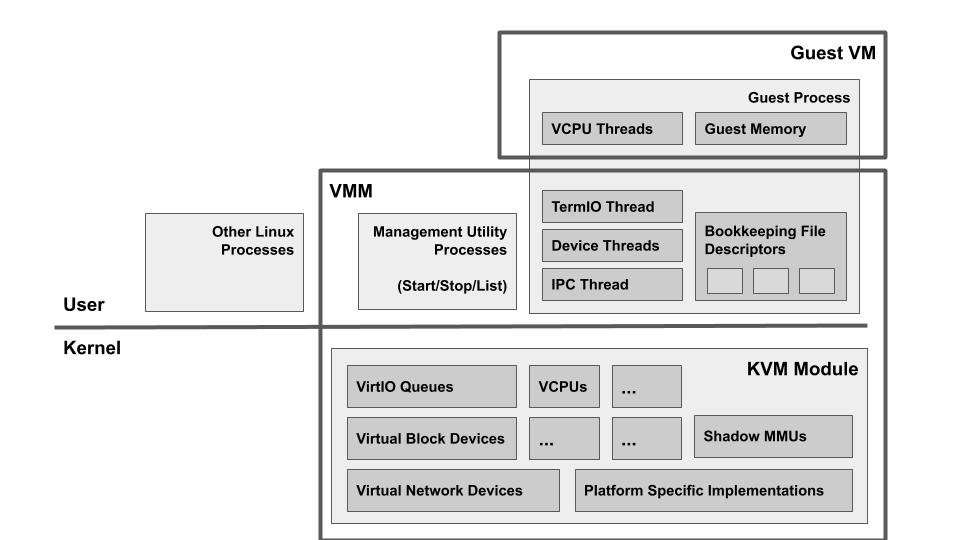
\includegraphics[width=0.8\textwidth]{{figures/kvm-arch}}
  \caption{KVM Software Architecture}
  \label{fig:kvm-arch}
\end{figure*}

\subsection{kvmtool}

kvmtool~\cite{kvmtool} is a VMM implementation for KVM with the minimal
functionality required to boot a fully functional linux kernel with very basic
virtualized devices. Supported devices include block, network, filesystem,
balloon, hardware random number generation, and console virtual devices, along
with a legacy 8250 serial device. kvmtool is provided as an alternative to
heavier VMM solutions such as QEMU~\cite{qemu}, which supports a wide range of
legacy devices and guest configurations.

We selected kvmtool as our userspace VMM as it offers a very similar set of
functionality to Firecracker, the VMM used to power Amazon Lambda. (TODO:
contrast firecracker and kvmtool) We chose kvmtool over Firecracker because we
found that Firecracker was more difficult to work with due to its Rust codebase
and containerization schemes. kvmtool provides a minimal platform on which to
test HyperFork applied to Linux guests and closely approximates the VMM of an
industrial serverless platform.

To virtualize efficiently, kvmtool makes use of a number of threads for
managing vCPUs and emulated devices. Userspace bookkeeping data structures hold
file descriptors which point to the internal VM state maintained within the KVM
kernel module. When the virtual machine is started, kvmtool creates a thread
for each class of device, including the terminal, 8250 serial console, block
devices, and other virtio devices. It then creates several worker threads to
handle arbitrary jobs that may arise from the virtio devices. These tasks
include processing work items from virtio queues and updating the console. In
its default configuration, kvmtool allocates one worker thread for each CPU on
the host machine. As we are virtualizing machines that are much smaller than
the host machine, we limited kvmtool to one worker thread per VM. In addition
to device threads, kvmtool also creates a thread to manage the virtual machines
through IPC calls. This allows administrators to start, pause, stop, and debug
virtual machines using a simple command line interface. Finally, kvmtool
creates one thread per vCPU that proceeds in a loop, invoking the
\texttt{KVM\_RUN} ioctl, then handling any IO requests or interrupts that may
arise. Together, this set of threads enables efficient virtualization of the
guest and its devices.

\section{Implementation}

We now describe the architecture and implementation of Hyperfork, along with
our design decisions regarding the flash-cloning operation.

For our KVM based virtualization platform, flash-cloning requires duplicating
several pieces of VM state. Where possible, we aim to make heavy use of the
linux fork operation to duplicate this state, as it is highly optimized and
provides copy-on-write functionality for duplicated pages. Specifically, guest
memory will be duplicated with copy-on-write functionality so that the backing
pages are not copied for the child unless necessary. However, fork leaves
kernelspace management state unduplicated, cannot duplicate all userspace VMM
threads, and leaves userspace bookkeeping file descriptors pointing to the
parent process's KVM management structures, which are inaccessible in the
child. Duplicating kernel state can either be performed within the kernel, by
coping in-kernel data structures, or in userspace by extracting and saving
guest specific state in userspace before forking. We predict a kernel
implementation may have slightly higher performance, but for simplicity we
implement our flash-cloning entirely in userspace within kvmtool.\footnote{Note
that a kernel implementation would also need to update file descriptors and
their memory mappings. This creates quite a mess in practice.} We also add an
ad-hoc guest-to-host communication channel with an extension to kvmtool to
enable our experimental evaluations.

\subsection{Flash-Cloning Support in kvmtool}

Our userspace HyperFork implementation for kvmtool proceeds in a series of
phases. At a high level, these phases are a triggering event, pre-fork
extraction and saving of kernel state, forking, and post-forking reconstruction
of VMM management state in the child.

First, the fork is triggered, either by an administrator invoking the
\texttt{FORK} IPC via the command line interface, or by the guest sending a
signal to the host indicating that it is ready to fork. In either case, the IPC
thread receives this signal, pauses the virtual machine, and calls the pre-fork
routines.

Because KVM state becomes inaccessible in the child process after the VMM has
forked, all kernel state that must be restored in the child needs to be
recorded by the parent before forking. Alternatively, this could be implemented
by IPC between the parent and child, in which the state is sent after the fork
is complete. We have adopted the former approach. The pre-fork routine thus
saves all individual vCPU state for all vCPUs (registers, interrupt
configuration), global vCPU state (interrupt configuration, clock), and then
locks all mutexes that must survive in the guest. Note that it is not necessary
for the pre-fork routine to save the memory of the virtual machine. As the
memory is mapped in the VMM process, it is unaffected by the fork system call
and remains accessible. It will, however, need to be remapped in the guest
following the fork.

Once the pre-fork routine is complete, kvmtool calls the system call fork. In
the parent, all of the locks acquired by the pre-fork routines are released and
execution proceeds. In the child, the post-fork routine is invoked, performing
the following to reconstruct necessary VMM state:

\begin{enumerate}
\item Acquires new file descriptors for the KVM device and virtual machine
\item Creates new file descriptors for the vCPUs
\item Restores individual and global vCPU state\footnote{In the process of
restoring this state, we encountered a bug in how KVM handles setting the
control registers when they change whether the guest is in long mode. We intend
to investigate this further and report it if necessary.}
\item Replaces all eventfds used for signalling
\item Creates new threads to handle devices and the execution of each vCPU
\item Releases all mutexes locked in the pre-fork routine, and replaces all
condition variables\footnote{Condition variables must be replaced, as in many
pthread implementations they contain an internal mutex that cannot be locked in
the pre-fork routine. If this mutex is locked by another thread when the IPC
thread performs the fork, the mutex will be permanently locked in the child
process.}
\item Attaches the terminal device to a new pseudo-terminal, or detaches it to
accept no further input\footnote{Due to a bug in kvmtool, operating with a
pseudoterminal with no slave is not supported.}
\end{enumerate}

Once the post-fork routine is complete, the vCPUs begin executing in the child
and the flash-clone operation is complete. We can also note that the original
thread in the parent which performed the forking operation was the IPC handling
thread. In the child, this thread creates a new IPC handling thread and then
assumes the role of the main kvmtool run thread, waiting on the guest vCPU0 to
exit and then terminating the VM gracefully.

\subsection{Guest-to-Host Signaling}

For guests with more complex forking behavior, the guest may need to inform the
host when it is ready to fork. For example, a virtual machine running a python
program may chose to fork on boot, after python has started, after modules are
loaded, or after further program initialization has completed. As the guest's
userspace state is very difficult to detect from the VMM, we implement a
rudimentary system for guest-to-host signaling.

The guest-to-host signal consists of sending a message over one of the
processor's ports. This allows for a simple and very efficient way to send
short messages to the host, without requiring any modifications to the guest
kernel. This functionality is accessible from userspace through the C standard
library. We define one message to indicate that the guest is ready to fork, and
one message to indicate that the guest has completed its task. To support our
evaluations, we include in the guest images a \texttt{fork} and \texttt{done}
executable that signal the two events which can be easily executed by guest
benchmarks. Further messages could easily be defined for a more complex
deployment.
